%%%%%%%%%%%%%%%%%%%%%%%%%%%%%%%%%%%%%%%%%%%%%%%%%%%%%%%%%%%%%%%%%%%%
%% I, the copyright holder of this work, release this work into the
%% public domain. This applies worldwide. In some countries this may
%% not be legally possible; if so: I grant anyone the right to use
%% this work for any purpose, without any conditions, unless such
%% conditions are required by law.
%%%%%%%%%%%%%%%%%%%%%%%%%%%%%%%%%%%%%%%%%%%%%%%%%%%%%%%%%%%%%%%%%%%%

\documentclass{beamer}
\usetheme[faculty=fi,logo=otinanai]{fibeamer}
\usepackage[utf8]{inputenc}
\usepackage[main=english]{babel}

%% These macros specify information about the presentation
\title{Introduction to Git} %% that will be typeset on the
\subtitle{GEO2020 - 15/12/2017} %% title page.
\author{Stelios Vitalis, Hugo Ledoux}
	
%% These additional packages are used within the document:
\usepackage{ragged2e}  % `\justifying` text
\usepackage{booktabs}  % Tables
\usepackage{tabularx}
\usepackage{tikz}      % Diagrams
\usetikzlibrary{calc, shapes, backgrounds, mindmap, trees}
\usepackage{smartdiagram}
\usepackage{amsmath, amssymb}
\usepackage{url}       % `\url`s
\usepackage{listings}  % Code listings
\lstset{language=[LaTeX]{TeX}}
\usepackage{minted}
\frenchspacing

\usepackage{pifont}% http://ctan.org/pkg/pifont

\definecolor{burntorange}{cmyk}{0,0.52,1,0}

\usepackage{subcaption}
\usepackage{gitdags}

\usetikzlibrary{decorations.pathmorphing}

\definecolor{bluport}{HTML}{21ADFD}
\definecolor{orgport}{HTML}{E37322}
\definecolor{pplport}{HTML}{4F21E9}
\definecolor{redport}{HTML}{701315}

\makeatletter
\renewcommand\fibeamer@includeLogo[1][]{}
\newcommand{\bftt}[1]{\textbf{\texttt{#1}}}
\newcommand{\comment}[1]{{\color[HTML]{008080}\textit{\textbf{\texttt{#1}}}}}
\newcommand{\cmd}[1]{{\color[HTML]{008000}\bftt{#1}}}
\newcommand{\bs}{\char`\\}
\newcommand{\cmdbs}[1]{\cmd{\bs#1}}
\newcommand{\lcb}{\char '173}
\newcommand{\rcb}{\char '175}
\newcommand{\cmdbegin}[1]{\cmdbs{begin\lcb}\bftt{#1}\cmd{\rcb}}
\newcommand{\cmdend}[1]{\cmdbs{end\lcb}\bftt{#1}\cmd{\rcb}}
\makeatother

\newcommand*\keystroke[1]{%
	\tikz[baseline=(key.base)]
	\node[%
	draw,
	fill=white,
	drop shadow={shadow xshift=0.25ex,shadow yshift=-0.25ex,fill=black,opacity=0.75},
	rectangle,
	rounded corners=2pt,
	inner sep=1pt,
	line width=0.5pt,
	font=\scriptsize\sffamily
	](key) {#1\strut}
	;
}
\newcommand{\keystrokebftt}[1]{\keystroke{\bftt{#1}}}

\newcommand{\cmark}{\ding{51}}%
\newcommand{\xmark}{\ding{55}}%

\begin{document}
  \frame{\maketitle}

  \AtBeginSection[]{% Print an outline at the beginning of sections
    \begin{frame}<beamer>
     % \frametitle{Outline for Section \thesection}
      \tableofcontents[currentsection]
    \end{frame}
}

	\section{Version Control}
\subsection{Why do we need it?}
\begin{frame}{Versioning and Collaboration}
\framesubtitle{The general concept}
It's useful because:
\begin{itemize}
	\item It tracks history of our work
	\item It allows us to work as a team
	\item It can be used to extract statistics about a project
\end{itemize}
\end{frame}

\begin{frame}{Is it really new?}
\framesubtitle{Cloud already uses it}
You have probably used it on documents if you use:
\begin{itemize}
\item Dropbox + MS Office
\item Google Drive + Google Docs
\item OneDrive + MS Office
\end{itemize}
\end{frame}

\subsection{What is it?}
\begin{frame}{Version Control System (VCS)}
\framesubtitle{Definition}

\begin{definition}
	\emph{Version Control is the \alert{management} of changes to documents, computer programs, large web sites, and other collections of information.}\footnote[frame]{Wikipedia}
\end{definition}
\end{frame}

\begin{frame}{Version Control System (VCS)}
\framesubtitle{Benefits}

A VCS:
\begin{itemize}
	\item keeps \alert{revisions}
	\item allows for \alert{true collaboration}
	\item encapsulates \alert{workflow} (e.g. track time, issues, project management)
\end{itemize}

\end{frame}

\begin{frame}{VCS vs Cloud}
\framesubtitle{Although not really a comparison}

\begin{table}[!b]
	{\carlitoTLF % Use monospaced lining figures
		\begin{tabularx}{\textwidth}{Xcc}
			& \textbf{VCS} & \textbf{Cloud} \\
			\toprule
			Revisions & Manual & Auto \\
			\textbf{Revision Information} \\
			Author & \cmark & \cmark \\
			Timestamp & \cmark & \cmark \\
			Message & \cmark & \alert{\xmark} \\
			\textbf{Collaboration} \\
			Sharing & \cmark & \cmark \\
			Concurrent working & \cmark & \alert{\textbf{?}} \\
			Branching & \cmark & \alert{\xmark} \\
			\bottomrule
	\end{tabularx}}
\end{table}

But don't be confused... It can't replace your cloud file storage!
\end{frame}

    \begin{frame}{VCS}
    \framesubtitle{Definitions}
    
    \begin{block}{Repository}
    	A storage location where all versions and information about them are stored.
    \end{block}

	\begin{block}{Workspace}
		The actual working directory of the user.
	\end{block}
\end{frame}

    \subsection{Architecture}
    
    \begin{frame}{Types of VCS}
    There are two types:
    \begin{itemize}
    	\item Centralised
    	\begin{itemize}
    		\item Subversion (SVN)
    		\item Microsoft Team Foundation Server (TFS)
    		\item Concurrent Versions System (CVS)
    	\end{itemize}
    	\item Distributed
    	\begin{itemize}
    		\item Git
    		\item Mercurial
    	\end{itemize}
    \end{itemize}
    \end{frame}
    
    \begin{frame}{Centralised}
    \framesubtitle{Architecture}
    
    A server is the only repository and every user has a workspace.
\begin{figure}
	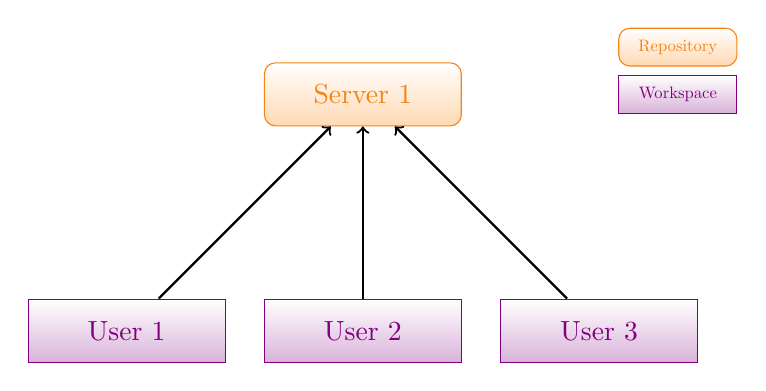
\begin{tikzpicture}
	\tikzstyle{repository}=[rectangle, draw, burntorange, rounded corners,
	thin,bottom color=orange!30, top color=white,
	text=burntorange, minimum width=2.5cm, minimum height=0.8cm]
	\tikzstyle{workspace} = [rectangle, draw, violet,
	thin,bottom color=violet!30, top color=white,
	text=violet, minimum width=2.5cm, minimum height=0.8cm]
	
	\node[repository] at (0,0) (server) {Server 1};
	\node[workspace] at (-3,-3) (user1) {User 1};
	\node[workspace] at (0,-3) (user2) {User 2};
	\node[workspace] at (3,-3) (user3) {User 3};
	
	\draw[thick, ->] (user1) -- (server);
	\draw[thick, ->] (user2) -- (server);
	\draw[thick, ->] (user3) -- (server);
	
	\node[repository, scale=0.6] at (4,0.6) {Repository};
\node[workspace, scale=0.6] at (4,0) {Workspace};
	
	\end{tikzpicture}
\end{figure}
\end{frame}

   \begin{frame}{Distributed}
\framesubtitle{Architecture}

No ``master'' server. Every user has a repository and a workspace.
\begin{figure}
	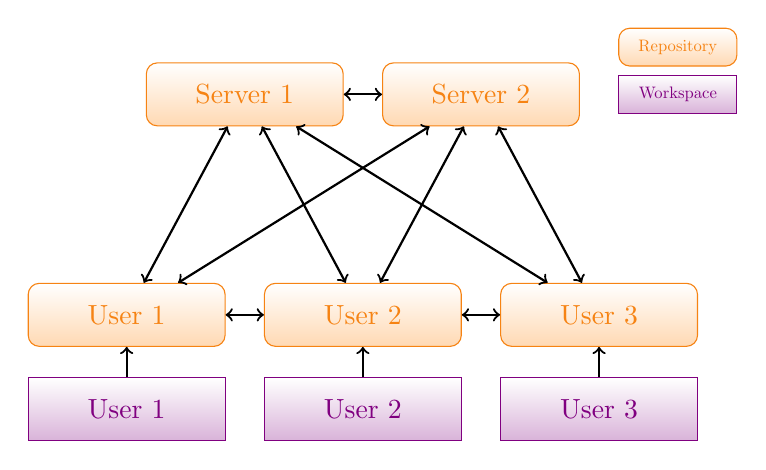
\begin{tikzpicture}
	\tikzstyle{repository}=[rectangle, draw, burntorange, rounded corners,
	thin,bottom color=orange!30, top color=white,
	text=burntorange, minimum width=2.5cm, minimum height=0.8cm]
	\tikzstyle{workspace} = [rectangle, draw, violet,
	thin,bottom color=violet!30, top color=white,
	text=violet, minimum width=2.5cm, minimum height=0.8cm]
	
	\node[repository] at (-1.5,0) (server1) {Server 1};
	\node[repository] at (1.5,0) (server2) {Server 2};
	\node[repository] at (-3,-2.8) (repo1) {User 1};
	\node[repository] at (0,-2.8) (repo2) {User 2};
	\node[repository] at (3,-2.8) (repo3) {User 3};
	\node[workspace] at (-3, -4) (ws1) {User 1};
	\node[workspace] at (0, -4) (ws2) {User 2};
	\node[workspace] at (3, -4) (ws3) {User 3};
		
	\draw[thick, <->] (repo1) -- (server1);
	\draw[thick, <->] (repo2) -- (server1);
	\draw[thick, <->] (repo3) -- (server1);
	
	\draw[thick, <->] (repo1) -- (server2);
	\draw[thick, <->] (repo2) -- (server2);
	\draw[thick, <->] (repo3) -- (server2);
	
	\draw[thick, <->] (server1) -- (server2);

	\draw[thick, <->] (repo1) -- (repo2);
	\draw[thick, <->] (repo2) -- (repo3);
	
	\draw[thick, ->] (ws1) -- (repo1);
	\draw[thick, ->] (ws2) -- (repo2);
	\draw[thick, ->] (ws3) -- (repo3);
	
	\node[repository, scale=0.6] at (4,0.6) {Repository};
	\node[workspace, scale=0.6] at (4,0) {Workspace};
	
	\end{tikzpicture}
\end{figure}
\end{frame}
    
    \subsection{Commits}
    \begin{frame}{Repository ``internals''}
      \framesubtitle{It's a graph}%
      \begin{figure}
      		\centering
      		\begin{tikzpicture}
      		% Commit DAG
      		\gitDAG[grow right sep = 2em]{
      			A -- B -- { 
      				C -- D,
      			}
      		};
      		\end{tikzpicture}
      \end{figure}
  
  This nodes are called \alert{commits} or \alert{revisions}.
    \end{frame}

    \begin{frame}{Commit or Revision}
\framesubtitle{Information}%
Every commit has:
\begin{itemize}
	\item \textbf{ID}: some short of identifier
	\item \textbf{Author}: \texttt{name} and \texttt{email} of user who commits
	\item \textbf{Timestamp}: \texttt{time} of commit
	\item \textbf{Message}: \texttt{what} the commit contains
\end{itemize}
and, of course, the \alert{changes} of the files that are submitted.
\end{frame}

\subsection{Branches}
\begin{frame}{Repository ``internals''}
\framesubtitle{Branching}%
\begin{figure}
	\centering
	\begin{tikzpicture}
	% Commit DAG
	\gitDAG[grow right sep = 2em]{
		A -- B -- { 
			C -- D,
		}
	};
	\gitbranch
	{master}     % node name and text 
	{above=of D} % node placement
	{D}          % target
	\end{tikzpicture}
\end{figure}
\end{frame}

\begin{frame}{Repository ``internals''}
\framesubtitle{Branching}%
\begin{figure}
	\centering
	\begin{tikzpicture}
	% Commit DAG
	\gitDAG[grow right sep = 2em]{
		A -- B -- C -- D -- { 
			E,
		}
	};
	\gitbranch
	{master}     % node name and text 
	{above=of D} % node placement
	{D}          % target
	\gitbranch
	{one-branch}
	{above=of E}
	{E}
	\end{tikzpicture}
\end{figure}
\end{frame}

\begin{frame}{Repository ``internals''}
\framesubtitle{Branching}%
\begin{figure}
	\centering
	\begin{tikzpicture}
	% Commit DAG
	\gitDAG[grow right sep = 2em]{
		A -- B -- C -- D -- { 
			F,
			E,
		}
	};
	\gitbranch
	{master}     % node name and text 
	{above=of F} % node placement
	{F}          % target
	\gitbranch
	{one-branch}
	{below=of E}
	{E}
	\end{tikzpicture}
\end{figure}
\end{frame}

\begin{frame}{Repository ``internals''}
\framesubtitle{Branching}%
\begin{figure}
	\centering
	\begin{tikzpicture}
	% Commit DAG
	\gitDAG[grow right sep = 2em]{
		A -- B -- C -- D -- { 
			F,
			E -- G -- H,
		}
	};
	\gitbranch
	{master}     % node name and text 
	{above=of F} % node placement
	{F}          % target
	\gitbranch
	{one-branch}
	{below=of H}
	{H}
	\end{tikzpicture}
\end{figure}
\end{frame}

\begin{frame}{Repository ``internals''}
\framesubtitle{Merging}%
\begin{figure}
	\centering
	\begin{tikzpicture}
	% Commit DAG
	\gitDAG[grow right sep = 2em]{
		C -- D -- { 
			F,
			E -- G -- H,
		} -- I
	};
	\gitbranch
	{master}     % node name and text 
	{above=of I} % node placement
	{I}          % target
	\end{tikzpicture}
\end{figure}
\end{frame}

\section{Git}

\subsection{Definitions}
\begin{frame}{Git}
\framesubtitle{Some History}
Git was created by Linus Torvalds in 2005 because there was no decent version control system to maintain the Linux kernel.

He described the tool as "the stupid content tracker".
\end{frame}

\begin{frame}{Git}
\framesubtitle{Some History}
He setup the following objectives:
\begin{itemize}
	\item Performance
	\item Take CVS as an example of what not to do; if in doubt, make the exact opposite decision
	\item Support a distributed, BitKeeper-like workflow
	\item Include very strong safeguards against corruption, either accidental or malicious
\end{itemize}
\end{frame}

\begin{frame}{Git}
\framesubtitle{Definitions}

It's an open-source destributed VCS.

Specific definitions:
\begin{itemize}
	\item Every commit has an ID which is its contents hash. E.g.: \texttt{2c7ae1b9865e58797ba326d2f7a115bebb034fd7}
	\item We call the ``current'' commit as \alert{\texttt{HEAD}}.
\end{itemize}

\end{frame}

\begin{frame}{Git}
\framesubtitle{Definitions}

\centering
\begin{tikzpicture}
% Commit DAG
\gitDAG[grow right sep = 2em]{
	c7e2daa -- 2c7ae1b -- { 
		3a5de77,
		1842e25 -- 1a2e54b,
	}
};
% Remote branch
\gitbranch    % node name
{master} % node text
{above=of 3a5de77}    % node placement
{3a5de77}             % target
% Branch
\gitbranch
{new-feature}     % node name and text 
{above=of 1a2e54b} % node placement
{1a2e54b}          % target
% HEAD reference
\gitHEAD
{above=of new-feature} % node placement
{new-feature}          % target
\end{tikzpicture}

\end{frame}

\begin{frame}{Git}
\framesubtitle{Definitions}

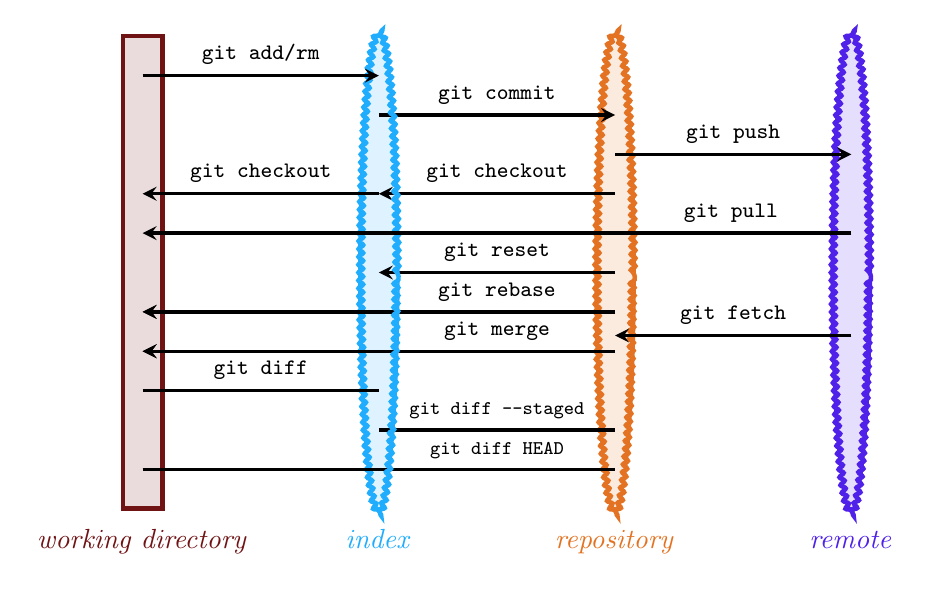
\begin{tikzpicture}

\fill[pplport!15] (12, 0) ellipse (0.25 and 3);
\fill[redport!15] (2.75, -3) rectangle (3.25, 3);
\fill[bluport!15] (6, 0) ellipse (0.25 and 3);
\fill[orgport!15] (9, 0) ellipse (0.25 and 3);

\draw[thick, pplport] (12, 0) ellipse (0.25 and 3);
\draw[ultra thick, pplport, decorate, decoration={snake, segment length=1mm, amplitude=0.3mm}] (12, 0) ellipse (0.23 and 3.05);
\node[text height=1em, text depth=1em, pplport] (1) at (12, -3.5) {\emph{remote}};

\draw[ultra thick, redport] (2.75, -3) rectangle (3.25, 3);
\node[text height=1em, text depth=1em, redport] (2) at (3, -3.5) {\emph{working directory}};

\draw[thick, orgport] (9, 0) ellipse (0.25 and 3);
\draw[ultra thick, orgport, decorate, decoration={snake, segment length=1mm, amplitude=0.3mm}] (9, 0) ellipse (0.23 and 3.05);
\node[text height=1em, text depth=1em, orgport] (4) at (9, -3.5) {\emph{repository}};

\draw[-stealth, very thick] (6, 2) -- node[above] {\tt\footnotesize git commit} (9, 2);
\draw[-stealth, very thick] (9, 1) -- node[above] {\tt\footnotesize git checkout} (6, 1);
\draw[-stealth, very thick] (9, 0) -- node[above] {\tt\footnotesize git reset} (6, 0);
\draw[very thick] (6, -2) -- node[above] {\tt\scriptsize git diff -{}-staged} (9, -2);
\draw[very thick] (3, -2.5) -- node[above, pos=0.75] {\tt\scriptsize git diff HEAD} (9, -2.5);
\draw[-stealth, very thick] (9, -0.5) -- node[above, pos=0.25] {\tt\footnotesize git rebase} (3, -0.5);
\draw[-stealth, very thick] (9, -1) -- node[above, pos=0.25] {\tt\footnotesize git merge} (3, -1);

% draw the blue portal here for the portal effect
\draw[thick, bluport] (6, 0) ellipse (0.25 and 3);
\draw[ultra thick, bluport, decorate, decoration={snake, segment length=1mm, amplitude=0.3mm}] (6, 0) ellipse (0.23 and 3.05);
\node[text height=1em, text depth=1em, bluport] (3) at (6, -3.5) {\emph{index}};

% Redraw some lines for piercing effect through blu port
\draw[-stealth, very thick] (6, -0.5) -- (3, -0.5);
\draw[-stealth, very thick] (6, -1) -- (3, -1);	
\draw[very thick] (3, -2.5) -- (6, -2.5);

\draw[-stealth, very thick] (3, 2.5) -- node[above] {\tt\footnotesize git add/rm} (6, 2.5);
\draw[-stealth, very thick] (9, 1.5) -- node[above] {\tt\footnotesize git push} (12, 1.5);
\draw[-stealth, very thick] (6, 1) -- node[above] {\tt\footnotesize git checkout} (3, 1);
\draw[-stealth, very thick] (12, 0.5) -- node[above, pos=0.17] {\tt\footnotesize git pull} (3, 0.5);
\draw[-stealth, very thick] (12, -0.8) -- node[above] {\tt\footnotesize git fetch} (9, -0.8);
\draw[very thick] (3, -1.5) -- node[above] {\tt\footnotesize git diff} (6, -1.5);
\end{tikzpicture}

\end{frame}

\subsection{Init or Clone}

\begin{frame}{Create a repository}
\framesubtitle{From scratch}

\begin{block}{	\texttt{git init}}
 	Creates a new empty repository.
 \end{block}

The \emph{working directory} is not affected, but an empty repository and index is created.

\end{frame}

\begin{frame}{Create a repository}
\framesubtitle{From a remote}

\begin{block}{	\texttt{git clone \emph{remote\_address}}}
	Creates a copy of an existing online repository.
\end{block}

\begin{itemize}
	\item A new folder is created.
	\item All commits/branches etc. are copied locally.
	\item The source repository is set as the \emph{origin} remote.
\end{itemize}

\end{frame}

\subsection{Add and Commit}

\begin{frame}{Status}
\framesubtitle{See where you stand}

\begin{block}{	\texttt{git status}}
	Gives all information about the current state of repository and index.
\end{block}

\begin{itemize}
	\item Shows current branch and difference with remote.
	\item Shows the staged files.
	\item Shows changed but not staged files.
	\item Shows untracked files.
\end{itemize}

\end{frame}

\begin{frame}{Create a commit}
\framesubtitle{Add files to the index}

\begin{block}{	\texttt{git add \emph{filename}}}
	Adds the file to the index. We say it's \alert{staged}.
\end{block}

\begin{itemize}
	\item The current file from \emph{working directory} is copied to the \emph{index} only if it has changes compared to HEAD.
	\item The \emph{filename} can be a pattern. Eg. ``\texttt{git add .}'' will add all files.
	\item Nothing has been committed yet.
\end{itemize}

\end{frame}

\begin{frame}{\texttt{git add file.txt}}
\begin{figure}
	\begin{subfigure}[b]{\textwidth}
		\centering
		\begin{tikzpicture}
		% Commit DAG
		\gitDAG[grow right sep = 2em]{
			c7e2daa -- 2c7ae1b -- { 
				{[nodes=unreachable] index -- {working dir} }
			}
		};
		% Branch
		\gitbranch
		{master}     % node name and text 
		{above=of 2c7ae1b} % node placement
		{2c7ae1b}          % target
		% Remote branch
		\gitremotebranch
		[origmaster]    % node name
		{file.txt} % node text
		{above=of {working dir}}    % node placement
		{{working dir}}             % target
		% HEAD reference
		\gitHEAD
		{above=of master} % node placement
		{master}          % target
		\end{tikzpicture}
		\subcaption{Before\ldots}
	\end{subfigure}
	
	\begin{subfigure}[b]{\textwidth}
		\centering
		\begin{tikzpicture}
		\gitDAG[grow right sep = 2em]{
	c7e2daa -- 2c7ae1b -- { 
		{[nodes=unreachable] index -- {working dir} }
	}
};
% Branch
\gitbranch
{master}     % node name and text 
{above=of 2c7ae1b} % node placement
{2c7ae1b}          % target
% Remote branch
\gitremotebranch
[filetxtindex]    % node name
{file.txt} % node text
{above=of {index}}    % node placement
{{index}}             % target
		% Remote branch
\gitremotebranch
[filetxtws]    % node name
{file.txt} % node text
{above=of {working dir}}    % node placement
{{working dir}}             % target
% HEAD reference
\gitHEAD
{above=of master} % node placement
{master}          % target
		\end{tikzpicture}
		\subcaption{\ldots{} and after}
	\end{subfigure}
\end{figure}
\end{frame}

\begin{frame}{Create a commit}
\framesubtitle{Commit staged files}

\begin{block}{	\texttt{git commit -m \emph{``message"}}}
	Creates a commit from a copy of the index.
\end{block}

\begin{itemize}
	\item The new commit has the given message.
	\item After the commit, the index is cleared.
	\item The \emph{HEAD} and the current \emph{branch} tags are moved to the new commit.
\end{itemize}

\end{frame}

\begin{frame}{\texttt{git commit -m "Changes to file.txt"}}
\begin{figure}
	\begin{subfigure}[b]{\textwidth}
		\centering
		\begin{tikzpicture}
		% Commit DAG
		\gitDAG[grow right sep = 2em]{
			c7e2daa -- 2c7ae1b -- { 
				{[nodes=unreachable] index -- {workspace} }
			}
		};
		% Branch
		\gitbranch
		{master}     % node name and text 
		{above=of 2c7ae1b} % node placement
		{2c7ae1b}          % target
		% Remote branch
		\gitremotebranch
		[origmaster]    % node name
		{file.txt} % node text
		{above=of index}    % node placement
		{index}             % target
				% Remote branch
		\gitremotebranch
		[filetxtws]    % node name
		{file.txt} % node text
		{above=of workspace}    % node placement
		{workspace}             % target
		% HEAD reference
		\gitHEAD
		{above=of master} % node placement
		{master}          % target
		\end{tikzpicture}
		\subcaption{Before\ldots}
	\end{subfigure}
	
	\begin{subfigure}[b]{\textwidth}
		\centering
		\begin{tikzpicture}
		\gitDAG[grow right sep = 2em]{
			c7e2daa -- 2c7ae1b -- 3a5de77 -- { 
				{[nodes=unreachable] index -- {workspace} }
			}
		};
		% Branch
		\gitbranch
		{master}     % node name and text 
		{above=of 3a5de77} % node placement
		{3a5de77}          % target
		% Remote branch
		\gitremotebranch
		[origmaster]    % node name
		{file.txt} % node text
		{below=of 3a5de77}    % node placement
		{3a5de77}             % target
		% HEAD reference
		\gitHEAD
		{above=of master} % node placement
		{master}          % target
		\end{tikzpicture}
		\subcaption{\ldots{} and after}
	\end{subfigure}
\end{figure}
\end{frame}

\subsection{Checkout}

\begin{frame}{Move to a commit}
\framesubtitle{Change branch or version}

\begin{block}{	\texttt{git checkout \emph{ref}}}
	Moves to a branch/commit and changes the working directory accordingly.
\end{block}

\begin{itemize}
	\item The \emph{ref} can be a branch name, commit id or something else...
	\item The \emph{HEAD} moves to the refered commit.
	\item The current branch changes (if a branch name is given).
\end{itemize}

\end{frame}

\begin{frame}{git checkout master}
\begin{figure}
	\begin{subfigure}[b]{\textwidth}
		\centering
		\begin{tikzpicture}
		% Commit DAG
		\gitDAG[grow right sep = 2em]{
			c7e2daa -- 2c7ae1b -- { 
				3a5de77,
				1842e25 -- 1a2e54b,
			}
		};
		% Remote branch
		\gitbranch    % node name
		{master} % node text
		{above=of 3a5de77}    % node placement
		{3a5de77}             % target
		% Branch
		\gitbranch
		{new-feature}     % node name and text 
		{above=of 1a2e54b} % node placement
		{1a2e54b}          % target
		% HEAD reference
		\gitHEAD
		{above=of new-feature} % node placement
		{new-feature}          % target
		\end{tikzpicture}
		\subcaption{Before\ldots}
	\end{subfigure}
	
	\begin{subfigure}[b]{\textwidth}
		\centering
		\begin{tikzpicture}
		% Commit DAG
		\gitDAG[grow right sep = 2em]{
			c7e2daa -- 2c7ae1b -- { 
				3a5de77,
				1842e25 -- 1a2e54b,
			}
		};
		% Remote branch
		\gitbranch    % node name
		{master} % node text
		{above=of 3a5de77}    % node placement
		{3a5de77}             % target
		% Branch
		\gitbranch
		{new-feature}     % node name and text 
		{above=of 1a2e54b} % node placement
		{1a2e54b}          % target
		% HEAD reference
		\gitHEAD
		{left=of master} % node placement
		{master}          % target
		\end{tikzpicture}
		\subcaption{\ldots{} and after. \alert{The working directory will change as well!}}
	\end{subfigure}
\end{figure}
\end{frame}

\begin{frame}{\texttt{git checkout 2c7ae1b}}
\begin{figure}
	\begin{subfigure}[b]{\textwidth}
		\centering
		\begin{tikzpicture}
		\gitDAG[grow right sep = 2em]{
			c7e2daa -- 2c7ae1b -- 3a5de77
		};
		% Branch
		\gitbranch
		{master}     % node name and text 
		{above=of 3a5de77} % node placement
		{3a5de77}          % target
		% Remote branch
		\gitremotebranch
		[origmaster]    % node name
		{file.txt} % node text
		{below=of 3a5de77}    % node placement
		{3a5de77}             % target
		% HEAD reference
		\gitHEAD
		{left=of master} % node placement
		{master}          % target
		\end{tikzpicture}
		\subcaption{Before\ldots}
	\end{subfigure}
	
	\begin{subfigure}[b]{\textwidth}
		\centering
		\begin{tikzpicture}
		\gitDAG[grow right sep = 2em]{
			c7e2daa -- 2c7ae1b -- 3a5de77
		};
		% Branch
		\gitbranch
		{master}     % node name and text 
		{above=of 3a5de77} % node placement
		{3a5de77}          % target
		% Remote branch
		\gitremotebranch
		[origmaster]    % node name
		{file.txt} % node text
		{below=of 3a5de77}    % node placement
		{3a5de77}             % target
		% HEAD reference
		\gitHEAD
		{above=of 2c7ae1b} % node placement
		{2c7ae1b}          % target
		\end{tikzpicture}
		\subcaption{\ldots{} and after. That's called a \alert{detached HEAD} state!}
	\end{subfigure}
\end{figure}
\end{frame}

\begin{frame}{\texttt{git checkout master}}
\begin{figure}
\begin{subfigure}[b]{\textwidth}
	\centering
	\begin{tikzpicture}
	\gitDAG[grow right sep = 2em]{
		c7e2daa -- 2c7ae1b -- 3a5de77
	};
	% Branch
	\gitbranch
	{master}     % node name and text 
	{above=of 3a5de77} % node placement
	{3a5de77}          % target
	% Remote branch
	\gitremotebranch
	[origmaster]    % node name
	{file.txt} % node text
	{below=of 3a5de77}    % node placement
	{3a5de77}             % target
	% HEAD reference
	\gitHEAD
	{above=of 2c7ae1b} % node placement
	{2c7ae1b}          % target
	\end{tikzpicture}
	\subcaption{Before on a `detached HEAD' state\ldots}
\end{subfigure}

\begin{subfigure}[b]{\textwidth}
	\centering
	\begin{tikzpicture}
	\gitDAG[grow right sep = 2em]{
		c7e2daa -- 2c7ae1b -- 3a5de77
	};
	% Branch
	\gitbranch
	{master}     % node name and text 
	{above=of 3a5de77} % node placement
	{3a5de77}          % target
	% Remote branch
	\gitremotebranch
	[origmaster]    % node name
	{file.txt} % node text
	{below=of 3a5de77}    % node placement
	{3a5de77}             % target
	% HEAD reference
	\gitHEAD
	{left=of master} % node placement
	{master}          % target
	\end{tikzpicture}
	\subcaption{\ldots{} and after. Back to normal.}
\end{subfigure}
\end{figure}
\end{frame}

\subsection{Branch and Merge}

\begin{frame}{Create a branch}
\framesubtitle{Use the branch command}

\begin{block}{	\texttt{git branch \emph{new-branch-name}}}
	Create a new branch here.
\end{block}

\begin{itemize}
	\item The new branch is created on the position of \texttt{HEAD}.
	\item The HEAD still points to the previous position.
\end{itemize}

\end{frame}

\begin{frame}{\texttt{git branch new-feature}}
\begin{figure}
	\begin{subfigure}[b]{\textwidth}
		\centering
		\begin{tikzpicture}
\gitDAG[grow right sep = 2em]{
	c7e2daa -- 2c7ae1b -- 3a5de77
};
% Branch
\gitbranch
{master}     % node name and text 
{above=of 3a5de77} % node placement
{3a5de77}          % target
% HEAD reference
\gitHEAD
{left=of master} % node placement
{master}          % target
\end{tikzpicture}
		\subcaption{Before\ldots}
	\end{subfigure}
	
	\begin{subfigure}[b]{\textwidth}
		\centering
		\begin{tikzpicture}
		\gitDAG[grow right sep = 2em]{
			c7e2daa -- 2c7ae1b -- 3a5de77
		};
		% Branch
		\gitbranch
		{master}     % node name and text 
		{above=of 3a5de77} % node placement
		{3a5de77}          % target
% Branch
\gitbranch
{new-feature}     % node name and text 
{above=of master} % node placement
{master}          % target
		% HEAD reference
		\gitHEAD
		{left=of master} % node placement
		{master}          % target
		\end{tikzpicture}
		\subcaption{\ldots{} and after.}
	\end{subfigure}
\end{figure}
\end{frame}

\begin{frame}{\texttt{git checkout new-feature}}
\begin{figure}
	\begin{subfigure}[b]{\textwidth}
		\centering
		\begin{tikzpicture}
		\gitDAG[grow right sep = 2em]{
			c7e2daa -- 2c7ae1b -- 3a5de77
		};
		% Branch
		\gitbranch
		{master}     % node name and text 
		{above=of 3a5de77} % node placement
		{3a5de77}          % target
		% Branch
		\gitbranch
		{new-feature}     % node name and text 
		{above=of master} % node placement
		{master}          % target
		% HEAD reference
		\gitHEAD
		{left=of master} % node placement
		{master}          % target
		\end{tikzpicture}
		\subcaption{Before\ldots}
	\end{subfigure}
	
	\begin{subfigure}[b]{\textwidth}
		\centering
		\begin{tikzpicture}
		\gitDAG[grow right sep = 2em]{
			c7e2daa -- 2c7ae1b -- 3a5de77
		};
		% Branch
		\gitbranch
		{master}     % node name and text 
		{above=of 3a5de77} % node placement
		{3a5de77}          % target
		% Branch
		\gitbranch
		{new-feature}     % node name and text 
		{above=of master} % node placement
		{master}          % target
		% HEAD reference
		\gitHEAD
		{left=of new-feature} % node placement
		{new-feature}          % target
		\end{tikzpicture}
		\subcaption{\ldots{} and after.}
	\end{subfigure}
\end{figure}
\end{frame}

\begin{frame}{Create a branch}
\framesubtitle{Use Checkout instead}

\begin{block}{	\texttt{git checkout -b \emph{new-branch-name}}}
	Create a new branch here and switch to it.
\end{block}

\begin{itemize}
	\item The new branch is created on the position of \texttt{HEAD}.
	\item The \texttt{HEAD} now points to the new branch.
\end{itemize}

\end{frame}

\begin{frame}{Merge branches}
\framesubtitle{There is a command for that}

\begin{block}{	\texttt{git merge \emph{other-branch}}}
	Merges the \emph{other-branch} to this one.
\end{block}

\begin{itemize}
	\item You call merge when you are on the branch that wants to ``receive'' the changes.
	\item Both branches remain after the merge, but changes have been incorporated to the current.
\end{itemize}

\end{frame}

\begin{frame}{git merge new-feature}
\begin{figure}
	\begin{subfigure}[b]{\textwidth}
		\centering
		\begin{tikzpicture}
		% Commit DAG
		\gitDAG[grow right sep = 2em]{
			c7e2daa -- 2c7ae1b -- { 
				3a5de77,
				1842e25 -- 1a2e54b,
			}
		};
		% Remote branch
		\gitbranch    % node name
		{master} % node text
		{above=of 3a5de77}    % node placement
		{3a5de77}             % target
		% Branch
		\gitbranch
		{new-feature}     % node name and text 
		{above=of 1a2e54b} % node placement
		{1a2e54b}          % target
		% HEAD reference
		\gitHEAD
		{left=of master} % node placement
		{master}          % target
		\end{tikzpicture}
		\subcaption{Before\ldots}
	\end{subfigure}
	
	\begin{subfigure}[b]{\textwidth}
		\centering
		\begin{tikzpicture}
		% Commit DAG
		\gitDAG[grow right sep = 2em]{
			c7e2daa -- 2c7ae1b -- { 
				3a5de77,
				1842e25 -- 1a2e54b,
			} -- 9ef2dad
		};
		% Remote branch
		\gitbranch    % node name
		{master} % node text
		{above=of 9ef2dad}    % node placement
		{9ef2dad}             % target
		% Branch
		\gitbranch
		{new-feature}     % node name and text 
		{right=of 1a2e54b} % node placement
		{1a2e54b}          % target
		% HEAD reference
		\gitHEAD
		{left=of master} % node placement
		{master}          % target
		\end{tikzpicture}
		\subcaption{\ldots{} and after. \alert{The working directory will change as well!}}
	\end{subfigure}
\end{figure}
\end{frame}

\begin{frame}{Conflict}

A conflict happens when during a merge there are changes to the same lines of the same document or when there is contradictory changes.

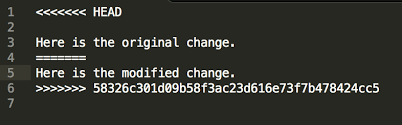
\includegraphics[width=\textwidth]{resources/conflict.png}

\begin{itemize}
	\item Both versions are shown.
	\item You change your files as normally.
	\item You add them again to the index.
	\item You commit.
\end{itemize}
\end{frame}

\begin{frame}{git merge new-feature}
\begin{figure}
	\begin{subfigure}[b]{\textwidth}
		\centering
		\begin{tikzpicture}
		% Commit DAG
		\gitDAG[grow right sep = 2em]{
			c7e2daa -- 2c7ae1b -- { 
				3a5de77,
				1842e25 -- 1a2e54b,
			}
		};
		% Remote branch
		\gitbranch    % node name
		{master} % node text
		{above=of 3a5de77}    % node placement
		{3a5de77}             % target
		% Branch
		\gitbranch
		{new-feature}     % node name and text 
		{above=of 1a2e54b} % node placement
		{1a2e54b}          % target
		% HEAD reference
		\gitHEAD
		{left=of master} % node placement
		{master}          % target
		\end{tikzpicture}
		\subcaption{Before\ldots}
	\end{subfigure}
	
	\begin{subfigure}[b]{\textwidth}
		\centering
		\begin{tikzpicture}
		% Commit DAG
		\gitDAG[grow right sep = 2em]{
			c7e2daa -- 2c7ae1b -- { 
				3a5de77,
				1842e25 -- 1a2e54b,
			} -- {[nodes=unreachable] index}
		};
		% Remote branch
		\gitbranch    % node name
		{master} % node text
		{above=of 3a5de77}    % node placement
		{3a5de77}             % target
		% Branch
		\gitbranch
		{new-feature}     % node name and text 
		{right=of 1a2e54b} % node placement
		{1a2e54b}          % target
		% HEAD reference
		\gitHEAD
		{left=of master} % node placement
		{master}          % target
		\end{tikzpicture}
		\subcaption{\ldots{} and after. \alert{The conflicts are marked and you have to resolvel!}}
	\end{subfigure}
\end{figure}
\end{frame}

\subsection{Remotes, Pull and Push}

\begin{frame}{Remotes}
\framesubtitle{The remote repositories}

\begin{block}{Remotes}
	A list of remote repositories that we can exchange commits.
\end{block}

\begin{itemize}
	\item Every \emph{remote} is reached through a url.
	\item It is given a \emph{name} to be distinguished.
	\item Normally we call the ``main'' remote as \alert{origin}.
\end{itemize}

\end{frame}

\begin{frame}{Fetch}
\framesubtitle{Get commits from remote}

\begin{block}{\texttt{git pull}}
	Fetches all commits from the remote and tries to merge the upstream to the current one.
\end{block}

\begin{itemize}
	\item Remember, remote branches are also branches, so they can be merged.
\end{itemize}

\end{frame}

\begin{frame}{git fetch origin}
\begin{figure}
	\begin{subfigure}[b]{\textwidth}
\centering
\begin{tikzpicture}
% Commit DAG
\gitDAG[grow right sep = 2em]{
	A -- B -- { 
		C,
	}
};
% Remote branch
\gitremotebranch
[origmaster]    % node name
{origin/master} % node text
{right=of C}    % node placement
{C}             % target
% Branch
\gitbranch
{master}     % node name and text 
{above=of C} % node placement
{C}          % target
% HEAD reference
\gitHEAD
{above=of master} % node placement
{master}          % target
\end{tikzpicture}
		\subcaption{Before\ldots}
	\end{subfigure}
	
	\begin{subfigure}[b]{\textwidth}
\centering
\begin{tikzpicture}
% Commit DAG
\gitDAG[grow right sep = 2em]{
	A -- B -- { 
		C -- D -- E,
	}
};
% Remote branch
\gitremotebranch
[origmaster]    % node name
{origin/master} % node text
{above=of E}    % node placement
{E}             % target
% Branch
\gitbranch
{master}     % node name and text 
{above=of C} % node placement
{C}          % target
% HEAD reference
\gitHEAD
{above=of master} % node placement
{master}          % target
\end{tikzpicture}
		\subcaption{\ldots{} and after.}
	\end{subfigure}
\end{figure}

\end{frame}

\begin{frame}{git fetch origin}
\begin{figure}
	\begin{subfigure}[b]{\textwidth}
\centering
\begin{tikzpicture}
% Commit DAG
\gitDAG[grow right sep = 2em]{
	A -- B -- { 
		D -- E,
	}
};
% Remote branch
\gitremotebranch
[origmaster]    % node name
{origin/master} % node text
{above=of B}    % node placement
{B}             % target
% Branch
\gitbranch
{master}     % node name and text 
{above=of E} % node placement
{E}          % target
% HEAD reference
\gitHEAD
{above=of master} % node placement
{master}          % target
\end{tikzpicture}
		\subcaption{Before\ldots}
	\end{subfigure}
	
	\begin{subfigure}[b]{\textwidth}
\centering
\begin{tikzpicture}
% Commit DAG
\gitDAG[grow right sep = 2em]{
	A -- B -- { 
		C,
		D -- E,
	}
};
% Remote branch
\gitremotebranch
[origmaster]    % node name
{origin/master} % node text
{above=of C}    % node placement
{C}             % target
% Branch
\gitbranch
{master}     % node name and text 
{above=of E} % node placement
{E}          % target
% HEAD reference
\gitHEAD
{above=of master} % node placement
{master}          % target
\end{tikzpicture}
		\subcaption{\ldots{} and after.}
	\end{subfigure}
\end{figure}

\end{frame}

\begin{frame}{Pull}
\framesubtitle{It's a fetch and merge}

\begin{block}{\texttt{git pull \emph{[remote-name]}}}
	Fetches all commits from the remote and merges.
\end{block}

\begin{itemize}
	\item It does \texttt{git fetch} and \texttt{git merge \emph{remote-name/branch}}
\end{itemize}

\end{frame}

\begin{frame}{git pull}
\begin{figure}
	\begin{subfigure}[b]{\textwidth}
		\centering
		\begin{tikzpicture}
		% Commit DAG
		\gitDAG[grow right sep = 2em]{
			A -- B -- { 
				C,
			}
		};
		% Remote branch
		\gitremotebranch
		[origmaster]    % node name
		{origin/master} % node text
		{right=of C}    % node placement
		{C}             % target
		% Branch
		\gitbranch
		{master}     % node name and text 
		{above=of C} % node placement
		{C}          % target
		% HEAD reference
		\gitHEAD
		{above=of master} % node placement
		{master}          % target
		\end{tikzpicture}
		\subcaption{Before\ldots}
	\end{subfigure}
	
	\begin{subfigure}[b]{\textwidth}
		\centering
		\begin{tikzpicture}
		% Commit DAG
		\gitDAG[grow right sep = 2em]{
			A -- B -- { 
				C -- D -- E,
			}
		};
		% Remote branch
		\gitremotebranch
		[origmaster]    % node name
		{origin/master} % node text
		{right=of E}    % node placement
		{E}             % target
		% Branch
		\gitbranch
		{master}     % node name and text 
		{above=of E} % node placement
		{E}          % target
		% HEAD reference
		\gitHEAD
		{above=of master} % node placement
		{master}          % target
		\end{tikzpicture}
		\subcaption{\ldots{} and after.}
	\end{subfigure}
\end{figure}

\end{frame}

\begin{frame}{git pull}
\begin{figure}
	\begin{subfigure}[b]{\textwidth}
		\centering
		\begin{tikzpicture}
		% Commit DAG
		\gitDAG[grow right sep = 2em]{
			A -- B -- { 
				D -- E,
			}
		};
		% Remote branch
		\gitremotebranch
		[origmaster]    % node name
		{origin/master} % node text
		{above=of B}    % node placement
		{B}             % target
		% Branch
		\gitbranch
		{master}     % node name and text 
		{above=of E} % node placement
		{E}          % target
		% HEAD reference
		\gitHEAD
		{above=of master} % node placement
		{master}          % target
		\end{tikzpicture}
		\subcaption{Before\ldots}
	\end{subfigure}
	
	\begin{subfigure}[b]{\textwidth}
		\centering
		\begin{tikzpicture}
		% Commit DAG
		\gitDAG[grow right sep = 2em]{
			A -- B -- { 
				C,
				D -- E,
			} -- F
		};
		% Remote branch
		\gitremotebranch
		[origmaster]    % node name
		{origin/master} % node text
		{above=of C}    % node placement
		{C}             % target
		% Branch
		\gitbranch
		{master}     % node name and text 
		{right=of F} % node placement
		{F}          % target
		% HEAD reference
		\gitHEAD
		{above=of master} % node placement
		{master}          % target
		\end{tikzpicture}
		\subcaption{\ldots{} and after.}
	\end{subfigure}
\end{figure}

\end{frame}

\begin{frame}{Push}
\framesubtitle{Share your changes to the world}

\begin{block}{\texttt{git push}}
	Push your local branch(es) to the remote.
\end{block}

\begin{itemize}
	\item Normally it just pushes the current branch to the upstream.
	\item Will only work if the remote branch is updated and there is a fast-forward to the local branch.
\end{itemize}

\end{frame}

\begin{frame}{git push}
\begin{figure}
	\begin{subfigure}[b]{\textwidth}
		\centering
		\begin{tikzpicture}
		% Commit DAG
		\gitDAG[grow right sep = 2em]{
			A -- B -- { 
				C -- {[nodes=unreachable] D -- E},
			}
		};
		% Remote branch
		\gitremotebranch
		[origmaster]    % node name
		{origin/master} % node text
		{above=of C}    % node placement
		{C}             % target
		% Branch
		\gitbranch
		{master}     % node name and text 
		{above=of E}% node placement
			{E}          % target
			% HEAD reference
			\gitHEAD
			{above=of master} % node placement
			{master}          % target
			\end{tikzpicture}
			\subcaption{Before\ldots}
		\end{subfigure}
		
		\begin{subfigure}[b]{\textwidth}
			\centering
			\begin{tikzpicture}
			% Commit DAG
			\gitDAG[grow right sep = 2em]{
				A -- B -- { 
					C -- D -- E,
				}
			};
			% Remote branch
			\gitremotebranch
			[origmaster]    % node name
			{origin/master} % node text
			{right=of E}    % node placement
			{E}             % target
			% Branch
			\gitbranch
			{master}     % node name and text 
			{above=of E} % node placement
			{E}          % target
			% HEAD reference
			\gitHEAD
			{above=of master} % node placement
			{master}          % target
			\end{tikzpicture}
			\subcaption{\ldots{} and after.}
		\end{subfigure}
	\end{figure}
	
\end{frame}

\begin{frame}{git push}
\begin{figure}
	\begin{subfigure}[b]{\textwidth}
		\centering
		\begin{tikzpicture}
		% Commit DAG
		\gitDAG[grow right sep = 2em]{
			A -- B -- { 
				C,
				{[nodes=unreachable] D -- E},
			} -- {[nodes=unreachable] F}
		};
		% Remote branch
		\gitremotebranch
		[origmaster]    % node name
		{origin/master} % node text
		{above=of C}    % node placement
		{C}             % target
		% Branch
		\gitbranch
		{master}     % node name and text 
		{right=of F} % node placement
		{F}          % target
		% HEAD reference
		\gitHEAD
		{above=of master} % node placement
		{master}          % target
		\end{tikzpicture}
		\subcaption{Before\ldots}
	\end{subfigure}
	
	\begin{subfigure}[b]{\textwidth}
		\centering
		\begin{tikzpicture}
		% Commit DAG
		\gitDAG[grow right sep = 2em]{
			A -- B -- { 
				C,
				D -- E,
			} -- F
		};
		% Remote branch
		\gitremotebranch
		[origmaster]    % node name
		{origin/master} % node text
		{above=of F}    % node placement
		{F}             % target
		% Branch
		\gitbranch
		{master}     % node name and text 
		{right=of F} % node placement
		{F}          % target
		% HEAD reference
		\gitHEAD
		{above=of master} % node placement
		{master}          % target
		\end{tikzpicture}
		\subcaption{\ldots{} and after.}
	\end{subfigure}
\end{figure}

\end{frame}

\begin{frame}{Git}
\framesubtitle{Overview}

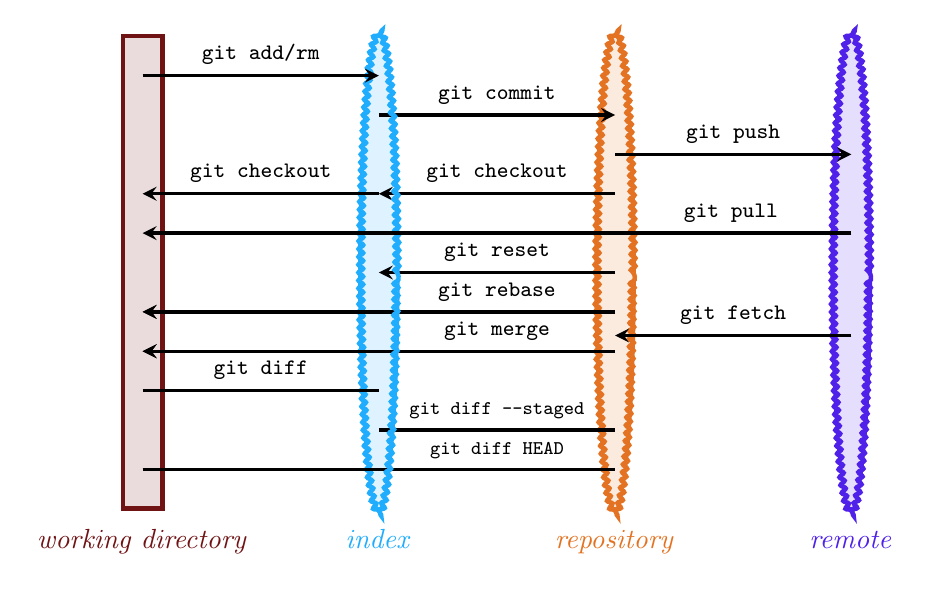
\begin{tikzpicture}

\fill[pplport!15] (12, 0) ellipse (0.25 and 3);
\fill[redport!15] (2.75, -3) rectangle (3.25, 3);
\fill[bluport!15] (6, 0) ellipse (0.25 and 3);
\fill[orgport!15] (9, 0) ellipse (0.25 and 3);

\draw[thick, pplport] (12, 0) ellipse (0.25 and 3);
\draw[ultra thick, pplport, decorate, decoration={snake, segment length=1mm, amplitude=0.3mm}] (12, 0) ellipse (0.23 and 3.05);
\node[text height=1em, text depth=1em, pplport] (1) at (12, -3.5) {\emph{remote}};

\draw[ultra thick, redport] (2.75, -3) rectangle (3.25, 3);
\node[text height=1em, text depth=1em, redport] (2) at (3, -3.5) {\emph{working directory}};

\draw[thick, orgport] (9, 0) ellipse (0.25 and 3);
\draw[ultra thick, orgport, decorate, decoration={snake, segment length=1mm, amplitude=0.3mm}] (9, 0) ellipse (0.23 and 3.05);
\node[text height=1em, text depth=1em, orgport] (4) at (9, -3.5) {\emph{repository}};

\draw[-stealth, very thick] (6, 2) -- node[above] {\tt\footnotesize git commit} (9, 2);
\draw[-stealth, very thick] (9, 1) -- node[above] {\tt\footnotesize git checkout} (6, 1);
\draw[-stealth, very thick] (9, 0) -- node[above] {\tt\footnotesize git reset} (6, 0);
\draw[very thick] (6, -2) -- node[above] {\tt\scriptsize git diff -{}-staged} (9, -2);
\draw[very thick] (3, -2.5) -- node[above, pos=0.75] {\tt\scriptsize git diff HEAD} (9, -2.5);
\draw[-stealth, very thick] (9, -0.5) -- node[above, pos=0.25] {\tt\footnotesize git rebase} (3, -0.5);
\draw[-stealth, very thick] (9, -1) -- node[above, pos=0.25] {\tt\footnotesize git merge} (3, -1);

% draw the blue portal here for the portal effect
\draw[thick, bluport] (6, 0) ellipse (0.25 and 3);
\draw[ultra thick, bluport, decorate, decoration={snake, segment length=1mm, amplitude=0.3mm}] (6, 0) ellipse (0.23 and 3.05);
\node[text height=1em, text depth=1em, bluport] (3) at (6, -3.5) {\emph{index}};

% Redraw some lines for piercing effect through blu port
\draw[-stealth, very thick] (6, -0.5) -- (3, -0.5);
\draw[-stealth, very thick] (6, -1) -- (3, -1);	
\draw[very thick] (3, -2.5) -- (6, -2.5);

\draw[-stealth, very thick] (3, 2.5) -- node[above] {\tt\footnotesize git add/rm} (6, 2.5);
\draw[-stealth, very thick] (9, 1.5) -- node[above] {\tt\footnotesize git push} (12, 1.5);
\draw[-stealth, very thick] (6, 1) -- node[above] {\tt\footnotesize git checkout} (3, 1);
\draw[-stealth, very thick] (12, 0.5) -- node[above, pos=0.17] {\tt\footnotesize git pull} (3, 0.5);
\draw[-stealth, very thick] (12, -0.8) -- node[above] {\tt\footnotesize git fetch} (9, -0.8);
\draw[very thick] (3, -1.5) -- node[above] {\tt\footnotesize git diff} (6, -1.5);
\end{tikzpicture}

\end{frame}

\section{Github and Workflow}

\begin{frame}{Github}
\framesubtitle{It's just a web app}
It's a repository hosting service, based on an closed-source web app that wraps git!

\begin{itemize}
	\item You can create remote repositories there (free for public, paid for private use).
	\item It incorporates some management tools as well (issue-tracking, pull requests, continuous integration).
\end{itemize}

There are other platforms out there as well, like Gitlab.
\end{frame}

\begin{frame}{Github}
\framesubtitle{Clone a repo}
\alert{\texttt{git clone https://github.com/qgis/QGIS.git}}

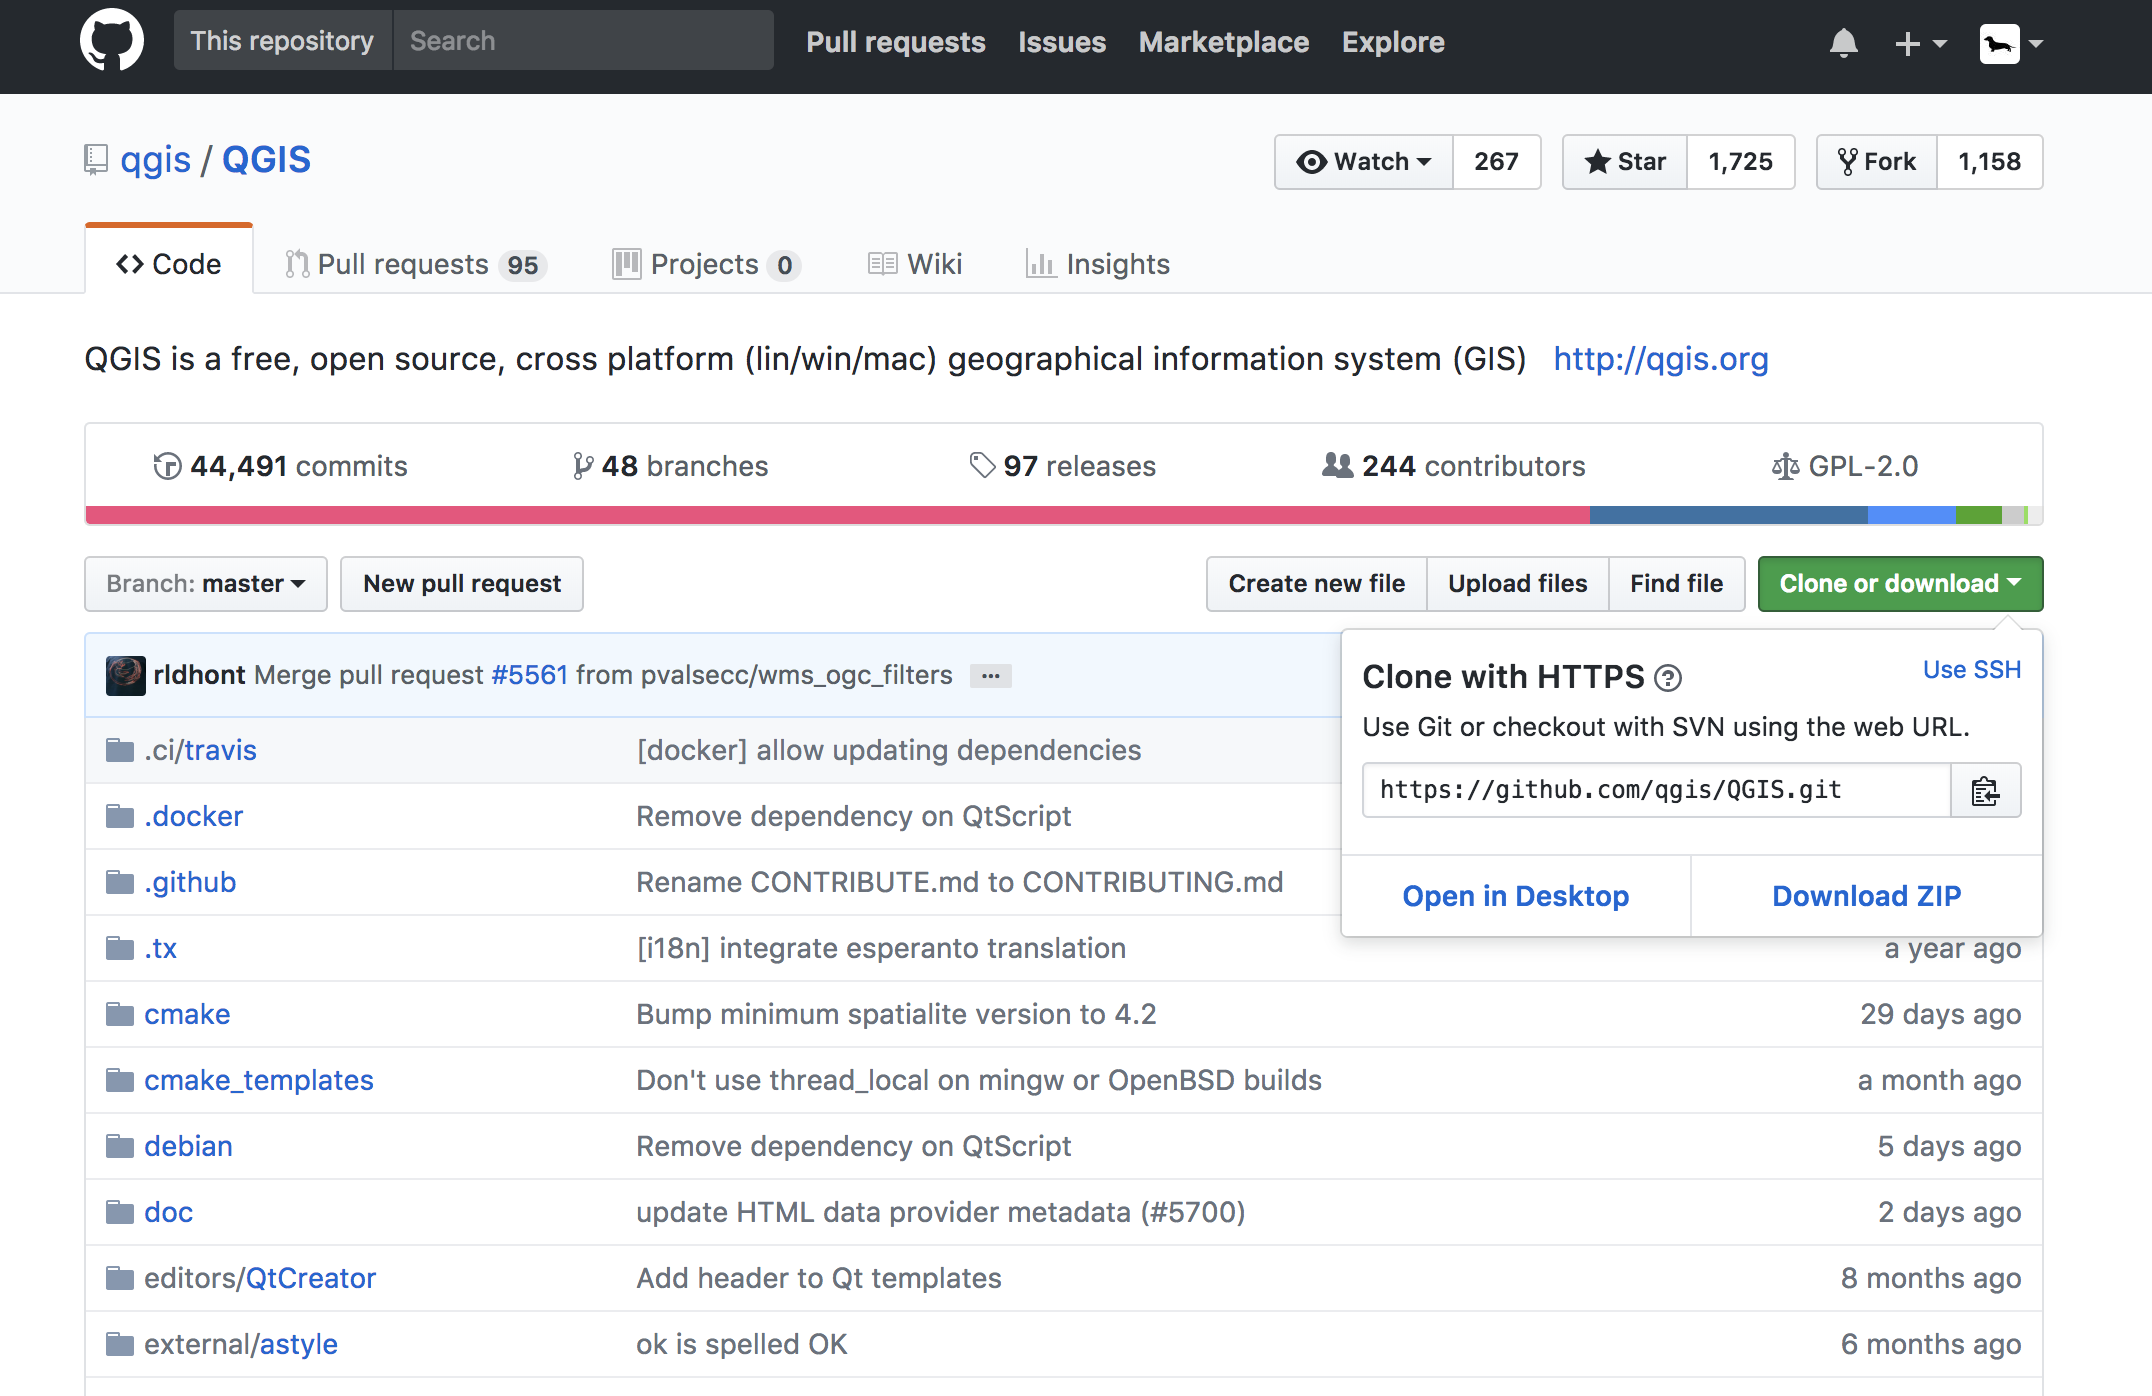
\includegraphics[width=\textwidth]{resources/github.png}
\end{frame}
    
\end{document}
